 %\renewcommand{\bottomfraction}{.7}
 %\renewcommand{\textfraction}{.15}
 %\renewcommand{\floatpagefraction}{.66}
 %\renewcommand{\dbltopfraction}{.66}
 %\renewcommand{\dblfloatpagefraction}{.66}
 %\setcounter{topnumber}{9}
 %\setcounter{bottomnumber}{9}
 %\setcounter{totalnumber}{20}
 %\setcounter{dbltopnumber}{9}

 
\newcommand{\makeBasicPlottingFig}{%
\begin{figure*}[tbh]
 \centering
% \includegraphics[width=\linewidth]{basicPlotting}
 \includegraphics[width=1.0\textwidth]{figures/basicPlotting.pdf}
 \caption{A selection of basic plots from PyQtGraph's suite of examples.}
 \label{fig:basicPlotting}
\end{figure*}}

\newcommand{\makePtreeExFig}{%
\begin{figure}[!htbp]
\centering
\includegraphics[width=\columnwidth]{figures/pg_ptree_ex}
\caption{Sample use of parameter trees for user interaction, where various image processing parameters can be quickly updated. The displayed image reflects these changes in real-time.}
 \label{fig:ptreeEx}
\end{figure}}

\newcommand{\makeNeuralNetFig}{%
\begin{figure*}
\centering
\includegraphics[width=0.8\textwidth]{figures/neuralNetFig}
\caption{Application demonstrating how parameter trees, real-time plotting updates, signal hooks, and more can facilitate rapid prototyping and impacts of architectural changes.}
 \label{fig:neuralNetFig}
\end{figure*}}

\newcommand{\makeLineBenchmarkFig}{%
\begin{figure}[!b]
\centering
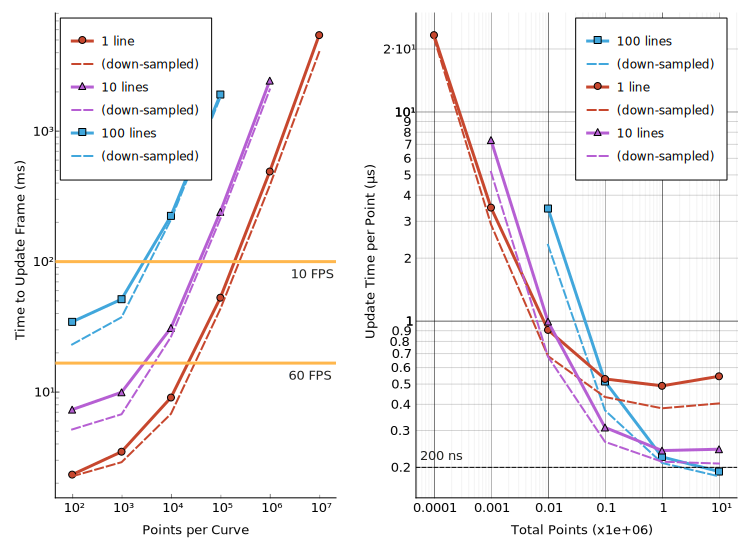
\includegraphics[width=\columnwidth]{figures/lineBenchmark}
\caption{Line speed benchmark. The time to render 1, 10 or 100 lines of data is shown for varying numbers of points per line. All data was collected on a 2020 MacBook Pro with i5 Processor. Left: Time per update over points per curve. The thresholds for achieving 10 and 60 frames/s are shown by horizontal lines. Right: Update time per point, plotted over the total number of points. For more than 100,000 points, the line-plotting time becomes dominant, and the results converge to 200\,ns per point for both 10 and 100 curves, while plotting all points as a single curve increases the time to 500--600 ns\,per point.}
 \label{fig:lineSpeed}
\end{figure}
}
 %13-inch 
 
\newcommand{\makeMatplotlibComparison}{%
\begin{figure}[bth]
\centering
\includegraphics[width=0.9\columnwidth]{figures/pg-mpl-comparison_no_interpolation.png}
\caption{Performance test with PyQtGraph and Matplotlib widgets embedded in a Qt5 application. Over a wide range of image sizes, PyQtGraph completes drawing approximately 75--150 times faster, taking only 5.4\,ms in this example of a 4000\texttimes4000 image. The test is performed without GPU acceleration in a Microsoft Windows environment, and both libraries are set to sub-sample without interpolation. Free-to-use test images are provided by the "Unsplash" service\cite{unsplash_license}.} 
\label{fig:mpl}
\end{figure}
}

 \newcommand{\makeARBBenchmarkFig}{
 \begin{figure}[tbh]
 \centering
 \includegraphics[width=\columnwidth]{figures/makeARGB_plot_revision_2.pdf}
 \caption{Image speed benchmark. The time to execute \texttt{makeARGB} for a single image  frame is shown for different data formats. Left: Using optimized NumPy processing (dashed lines), the drawing time is log-scale linear with the number of pixels over a wide range. GPU accelerated CUDA processing (solid lines) describe a more complex relationship with image size. The need to copy data to and from the GPU creates additional overhead, but as image size grows, the faster processing speed becomes sufficient to compensate for that overhead. The choice of various extra processing tasks like LUTs or scaling (colors and shaded interval) show the same basic trends. The GPU offers a more significant improvement for the more complex image processing (blue). Right: For input data in uint16 format, CUDA processing is particularly advantageous and can provide an almost four-fold reduction in drawing time. Benchmarks were performed on an Intel i7-9750H processor at 2.60 GHz and an NVIDIA GeForce GTX 1660 Ti discrete GPU.}
 \label{fig:makeARGB}
 \end{figure}
 }
 
\newcommand{\makeMonitoringFig}{%
\begin{figure}[!htbp]
\centering
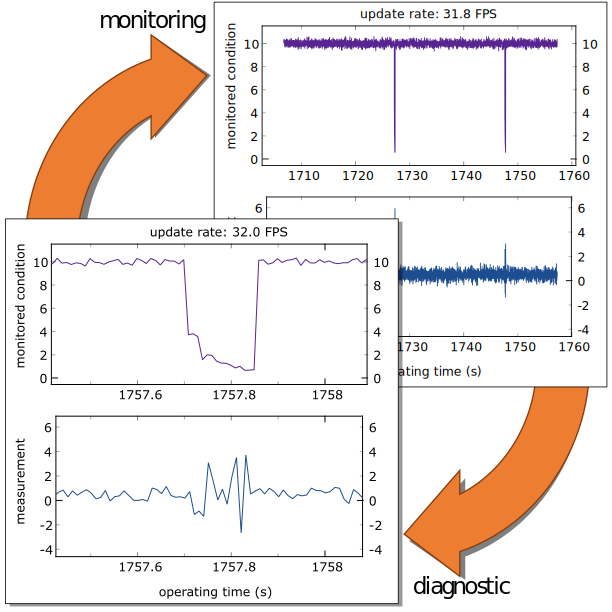
\includegraphics[width=\columnwidth]{figures/monitoring_example_vector.pdf}
\caption{Monitoring and diagnostic of a (simulated) experiment with intermittent failures. Incoming data at 100 samples/s for two measurement channels is recorded into a rolling 5,000 point buffer and continuously displayed at 30 frames/s. When a failure is observed, it can quickly be brought into focus with simple mouse interactions (click-and-drag and mousewheel zoom) for inspection, or to record accurate time stamps. Afterwards, a single click returns the view to automatic scaling without loss of any incoming data.}
 \label{fig:monitoring}
\end{figure}
}

